\documentclass[balance=false, sigconf]{acmart}

% ===== Don't touch this :) ======
\settopmatter{printacmref=false} % Removes citation information below abstract
\renewcommand\footnotetextcopyrightpermission[1]{} % removes footnote with conference information in first column
\renewcommand\footnotetextauthorsaddresses[1]{}
\pagestyle{plain} % removes running headers

\usepackage{graphicx}
\usepackage{amsmath}
\usepackage[algo2e]{algorithm2e}
\usepackage{algorithm}
\usepackage{algpseudocode}
\graphicspath{ {./images/} }
\usepackage{url}
\begin{document}
\title{Query-driven compaction in LSM-trees}

\author{Nishil Agrawal}
\affiliation{%
    \institution{Boston University}
    \country{}
}
\author{Shubham Kaushik}
\affiliation{%
    \institution{Boston University}
    \country{}
}
\author{Konstantinos Karatsenidis}
\affiliation{%
    \institution{Boston University}
    \country{}
}


\begin{abstract}
\textit{Log-structured merge-trees (LSM-trees)\cite{oneil1996logstructured, dayan2017monkey} have become a widely used data structure 
for persistent storage of key-value entries, particularly in write-intensive workloads. 
However, current LSM-tree designs do not capitalize on the sort-merge operations performed 
for range queries, leading to redundant work for range query-heavy workloads. In this 
research project, we aim to investigate and develop a range query-driven compaction approach 
for LSM-trees, focusing on enhancing the efficiency of range query processing and improving 
overall system performance for specific types of workloads. The proposed solution will 
involve understanding and configuring RocksDB's internal tunable parameters, designing innovative query-driven 
compaction algorithms, implementing a proposed solution, and benchmarking its
performance. Eager compaction can be performed based on incoming range queries to improve the performance of subsequent range queries. By implementing a smart range query-driven compaction strategy, it is possible 
to reduce I/O operations, CPU computation cycles, and improve space, write, and read 
amplification, leading to better system performance.}
\end{abstract}

\maketitle
\pagestyle{plain}

% =============================================================================
\section{Introduction}
% =============================================================================

Log-structured merge-trees (LSM-trees) are a widely used data structure for the persistent storage of key-value entries, excelling in write-intensive workloads. However, current LSM-tree designs do not fully exploit the potential of range query-heavy workloads, leading to redundant work and suboptimal performance. This research project aims to address this issue by investigating and developing a range query-driven compaction approach for LSM-trees to enhance range query processing efficiency and improve overall system performance for specific types of workloads.

Our approach involves understanding RocksDB's\cite{rocksdb} internal tunable parameters, designing innovative query-driven compaction algorithms, implementing the proposed solutions, and benchmarking their performance. By implementing a smart range query-driven compaction strategy, we can reduce I/O operations, CPU computation cycles, and improve space, write, and read amplification, resulting in better system performance.

This report is organized as follows: Section 1 introduces the motivations and the problem statement of this research project. Section 2 talks about the potential benefits of range query based compaction. Section 3 discusses potential approaches to solving the problems and introduces our proposed range query-driven compaction algorithm that attempts to solve the problem. Section 4 describes the experimental setup and results, followed by a discussion on the implications of our findings. We discuss the challenges we faced while working on this project in section 5. Finally, we discuss future work and conclude the report in Sections 6 and 7.


\subsection{Motivation}

LSM-trees store data on the disk as immutable logs or sorted sequence tables (SSTs), 
arranged in hierarchical levels of increasing capacity. In order to limit the number 
of logs that a lookup must probe, LSM-trees periodically perform sort-merge operations 
on logs of similar sizes, a process known as compaction.

Compaction in LSM-trees is primarily driven by the ingestion of new entries into the 
tree. Meanwhile, range queries merge all qualifying runs with overlapping key ranges, 
excluding older and logically invalidated entries. However, state-of-the-art 
LSM-tree designs do not capitalize on the sort-merge operations performed for the range 
queries by incorporating the results into the tree. This oversight can lead to 
redundant work for range query-heavy workloads, especially when the same range queries are 
executed multiple times.

By introducing a smart range query-driven compaction strategy, it is possible to reduce 
the number of I/O operations and CPU computation cycles required for the subsequent range 
queries, particularly those with overlapping ranges. This approach offers several 
potential benefits, including:

\begin{itemize}
    \item \textbf{Reduced space amplification}: By removing logically invalidated 
    entries, the overall storage footprint can be decreased.
    \item \textbf{Amortized write amplification}: By avoiding unnecessary writes during 
    compaction triggered by policy-driven approaches, the number of write operations 
    can be minimized.
    \item \textbf{Diminished read amplification}: By leveraging the improvements in 
    space and write amplification, the number of read operations for point lookups 
    can be reduced.
\end{itemize}

This research project proposal aims to investigate and develop a query-driven compaction 
approach for LSM-trees, focusing on enhancing the efficiency of range query processing 
and improving overall system performance for specific types of workloads.

\subsection{Problem Statement}

The primary objective of this project is to enable range query-driven compaction in LSM-trees, 
a topic that has not been extensively researched thus far. While existing research has 
primarily focused on optimizing compaction by modifying compaction policies, it has not 
specifically addressed range query-driven compaction. To explore the feasibility and potential 
benefits of this approach, we began by examining the RocksDB source code and analyzing its 
implementation of range queries.

In RocksDB, the \textbf{\textit{Seek(const Slice\& target)}} method of the \textbf{\textit{Iterator}} \cite{rocksdbiterator}
class performs a random walk on each level for every range query, returning an iterator for 
each level to initiate the sort-merge process. During this process, RocksDB merges the data 
with same keys from different levels and returns to the user valid records that fall within the 
queried range.

Two potential optimization opportunities arise when a range query is received from the application:

\begin{enumerate}
    \item An efficient algorithm can be executed with every range query, filtering out all 
files that can be compacted using the meta-data stored 
for SST files across all \textit{levels}, including \textit{memtables \& immutable memtables}
and calling a manual compaction using \textit{CompactFiles(vector<string> input\_file\_names)}, an in-built function provided by 
RocksDB. This filtering process can be based on several factors, such as the size of the files and the amount of key overlap between them. This approach will reduce \textit{space \& write 
amplification} by compacting files and storing them in lower levels.

\item An optimization opportunity arises after RocksDB has merged the keys within all the files of a subrange for the results of a range query. We can utilize the 
results of the range query to perform compaction and write them back to a higher level, thereby reducing 
the overhead of reading multiple files for other similar range queries. By intelligently leveraging 
the output generated during the range query, we can optimize the compaction process and minimize the 
work required for subsequent overlapping range queries.
\end{enumerate} 

Achieving this optimization requires a comprehensive understanding of the state-of-the-art compaction 
policies, the mechanisms that trigger compaction, and the steps involved in compaction between two or 
more levels. Additionally, it demands a more fine-grained approach to compaction that can accommodate 
different types of workloads. In summary, the problem to be addressed in this research project is developing and evaluating a range of query-driven compaction strategies for LSM-trees, aimed at improving 
compaction efficiency and overall system performance for specific workloads.

\subsection{Contributions}

The following are the key contributions of this research project on 
query-driven compaction in LSM-trees:
\begin{itemize}
    \item \textbf{Understanding RocksDB's internal tunable parameters}: Exploring 
    RocksDB's internal tunable parameters, focusing on how to optimize them for a 
    range operation-heavy workload. This will involve delving into the intricacies 
    of RocksDB's implementation and exploring ways to enhance its efficiency for range queries.
    \item \textbf{Design of query-driven compaction algorithms}: Developing innovative 
    query-driven compaction algorithms that use the metadata of files to perform manual compaction or take the advanatge of the sort-merge operations
     performed for range queries. These algorithms aim to help reduce the overhead of 
     range queries because of the amount duplicate keys by minimizing their occurrence.
    \item \textbf{Implementation of proposed solutions}: Implementing the proposed query-driven 
    compaction solution on top of RocksDB and conducting analysis on it. This 
    implementation will involve integrating one of the proposed algorithms into the existing 
    RocksDB architecture and ensuring their compatibility with the database's internal 
    tunable parameters. The implementation will be designed to enhance the efficiency of 
    range queries related to duplicates and provide a seamless experience for users.
    \item \textbf{Benchmarking and optimization}: Performing extensive benchmarking tests 
    using range operation-heavy workloads to evaluate and refine the implemented solutions. 
    These tests will involve comparing different approaches, tunable parameters, and their 
    effects on the overall performance of the query-driven compaction algorithms. The 
    benchmarking results will provide valuable insights into the strengths and weaknesses 
    of the proposed solutions and guide future refinements and enhancements.
\end{itemize}

% =============================================================================
\section{Background}
% =============================================================================

Although there has been limited research on query-driven compaction in LSM trees, it is 
essential to understand the potential benefits of eliminating duplicates to improve the 
read cost of range queries. 
We assume that all duplicates in a range are removed after the first range query is 
performed, and the subsequent range query is a subset of the previous range query. 
This analysis considers the following parameters for an LSM tree:

\begin{itemize}
\item $T$: Size ratio between adjacent levels
\item $L$: Number of levels
\item $P$: Number of disk pages in the buffer
\item $D$: Amount of duplicate keys
\item $S$: Selectivity of Range Query
\end{itemize}

By analyzing the number of pages accessed per level, the number of pages accessed due to 
duplicates, and the total number of pages accessed (including duplicates), we can estimate 
the potential improvement in range query performance after removing duplicates.

The number of pages accessed per level is given by:
\begin{equation}
  \sum_{l=0}^{l=L} S * P * T^l
\end{equation}

The number of pages accessed because of duplicates is:
\begin{equation}
  D * \sum_{l=0}^{l=L} S * P * T^l
\end{equation}

The total number of pages accessed, including duplicates, is:
\begin{equation}
  (1 + D) * \sum_{l=0}^{l=L} S * P * T^l
\end{equation}

The improvement is calculated as the relative reduction in cost between the old 
and new cost, as follows:

\begin{equation}
Improvement = \frac{OldCost-NewCost}{OldCost}
\end{equation}

The old cost is $1 + D$, and the new cost is $1$. Therefore, the improvement 
can be expressed as a ratio:

\begin{equation}
Improvement = \frac{(1 + D) - 1}{(1 + D)} = \frac{D}{(1 + D)}
\end{equation}

To convert the improvement into a percentage, multiply the ratio by 100:

\begin{equation}
ImprovementPercentage = \frac{D}{(1 + D)} * 100\%
\end{equation}

For example, if the duplication is 20\% of the entire data, we can estimate the 
potential improvement in range query performance after removing duplicates. 
Using the formula:
\begin{equation}
ImprovementPercentage = \frac{0.2}{(1 + 0.2)} * 100\% = 16.67\%
\end{equation}

Therefore, if the duplication is 20\% of the entire data, removing duplicates 
can potentially improve the range query performance by 16.67\%. This percentage 
of improvement is relatively small but can still be significant in scenarios 
where range queries are performed frequently or on large datasets. It is important 
to note that the improvement percentage will vary depending on the amount of 
duplication in data. As the amount of duplication increases, the potential 
improvement in range query performance will also increase.

% =============================================================================
\section{Architecture}
% =============================================================================

In LSM-trees, a single range query performs numerous operations before providing 
results to the user. The LSM-tree first hops to each level, identifies all keys 
within the queried range $[k_\text{min}, k_\text{max}]$, and performs a sort-merge 
to exclude logically invalidated keys or older entries. For large ranges and repeated 
range queries, this process involves redundant work. Our goal is to perform this 
task once for the entire range and subsequently only for valid keys in later queries.

Since we already perform the sort-merge operation after reading all the relevant 
pages, we can implement a smarter approach to writing them back after returning 
the results to the user. This requires an efficient algorithm to identify overlapping 
files between two or more levels.

We propose two approaches to tackle this problem:

\begin{enumerate}
    \item \textbf{Eager Compaction based on Range Query}: This approach involves eagerly triggering compaction by providing the files and levels that can be compacted based on the query range. This may require pulling these files back into memory according to the state-of-the-art compaction strategy and writing them back to the lower level. This approach can be tuned based on multiple parameters like range size, and the number of overlapping files. The can be achieved using \textit{CompactFiles(vector<string> input\_file\_names)} functionality after running an algorithm.
    
    \item \textbf{Intelligent Iterator}: When in-range files are pulled into the memory during a range-query operation, we can use the metadata of each file to know how much overlapping is occurring. If a file at level $x$ ($L_\text{x}$) overlaps entirely with a file at level $x+1$ ($L_\text{x+1}$), the result of the range query can be written to the file at level $L_\text{x+1}$, and the file at level $L_\text{x}$ page can be marked for garbage collection. This process can be applied across multiple levels, depending on the overlapping ranges. The iterator algorithm for the range query can be made to be worked intelligently to enable this set of tasks efficiently based on multiple parameters.
\end{enumerate}

The second algorithm is more complex than the first one. In the first algorithm, we are not using the results of the range query directly but rather marking the files, that have been accessed to generate the output of the range query, for compaction. While, in the second algorithm, we aim to directly use the iterators that generate the output for the range query to perform a set of functions on the tree for compaction while marking duplicates for garbage collection. 

\subsection{Solution Design}
As discussed in Section 3, we have two approaches for query-driven compaction. The high-level algorithms for these approaches are described below.

\textbf{Eager Compaction based on Range Query}
\begin{enumerate}
\item Execute the range query $[k_\text{min}, k_\text{max}]$ on the LSM-tree.
\item Identify all the files and corresponding levels that were accessed during the range query.
\item Calculate the degree of overlapping between the accessed files across levels.
\item Set a threshold for the range size and the number of overlapping files. If the overlapping degree exceeds the threshold, proceed with the eager compaction.
\item For each pair of overlapping files, read the data from the higher-level file and merge it with the lower-level file according to the state-of-the-art compaction strategy.
\item Write the merged data back to the lower level and delete the compacted file from the higher level.
\item Repeat steps 5-6 for each pair of overlapping files until all files have been compacted.
\item Update the LSM-tree metadata to reflect the changes.
\end{enumerate}

\textbf{Intelligent Iterator}
\begin{enumerate}
\item Execute the range query $[k_\text{min}, k_\text{max}]$ on the LSM-tree and store the accessed files and their metadata.
\item For each file at level $L_\text{x}$, check if it overlaps entirely with a file at level $L_\text{x+1}$.
\item If there is complete overlap, identify the lowest level among consecutive levels with overlapping files (e.g., $L_\text{x+n}$).
\item Combine the in-memory iterators for the range query result and the overlapping files from levels $L_\text{x+1}$ to $L_\text{x+n}$.
\item Write the merged iterator result back to the file at the lowest level, $L_\text{x+n}$.
\item Mark the files at levels $L_\text{x}$ to $L_\text{x+n-1}$ for garbage collection and update the LSM-tree metadata.
\item Repeat steps 2-6 for all files across multiple levels.
\item Remove the marked files and reclaim storage space by periodically performing garbage collection.
\end{enumerate}

\subsection{Pseudocode}
In this section, we present the Range Query Driven Compaction algorithm, an efficient approach to manage data in a multi-level storage system. 
This algorithm operates on file metadata to identify the relevant files that can be compacted within a specific key range and triggers a manual 
compaction process accordingly.

\begin{algorithm}
    \raggedright
    \SetAlgoLined
    \KwResult{Range Query Driven Compaction}
    
    \SetKwFunction{RangeQueryDrivenCompaction}{RangeQueryDrivenCompaction}
    \SetKwFunction{GetHighestLevelFromCompact}{GetHighestLevelFromCompact}
    \SetKwFunction{FilterFileThatCanBeCompacted}{FilterFileThatCanBeCompacted}
    \SetKwFunction{FilterOnlyInRangeFiles}{FilterOnlyInRangeFiles}
    \SetKwFunction{FilesToBeCompactedAcrossLevels}{FilesToBeCompactedAcrossLevels}
    \SetKwFunction{HighestFilesSizeAcrossLevels}{HighestFilesSizeAcrossLevels}
    \BlankLine

    \RangeQueryDrivenCompaction{$start\_key$, $end\_key$} \\
    Initialize column family handle, data, and version \\
    Create a vector of CompactionInputFiles for each non-empty level \\
    Combine level and file metadata collection loops \\
    $filter\_files \gets$ \FilterFileThatCanBeCompacted{$all\_files$, $start\_key$, $end\_key$, $cfd\_$} \\
    \If{$filter\_files.size() > 0$}{
        $level\_to\_write \gets$ \GetHighestLevelFromCompact{$filter\_files$} \\
        Create a list of input file names \\
        Perform compaction with the list of input file names at $level\_to\_write$ \\
    }
    \BlankLine

    \GetHighestLevelFromCompact{$files$} \\
    $max\_level \gets -1$ \\
    \ForEach{$cif \in files$}{
        Update $max\_level$ if $cif.level > max\_level$
    }
    \BlankLine

    \FilterFileThatCanBeCompacted{$all\_files$, $start\_key$, $end\_key$, $cfd\_$} \\
    Initialize variables and data structures \\
    Iterate files from last level to first \\
    Determine the largest and smallest key ranges \\
    Handle edge cases and track levels \\
    \Return {Files with the highest size across levels} \\
    \BlankLine

    \HighestFilesSizeAcrossLevels{$files\_to\_be\_compacted$} \\
    $max\_size \gets 0$ \\
    $index\_having\_largest\_size \gets -1$ \\
    \ForEach{$vec\_cif \in files\_to\_be\_compacted$}{
        Calculate the total size of files \\
        Update the index with the largest size \\
    }
    \Return{Files at the index with the largest size} \\
    \BlankLine
    
    \FilterOnlyInRangeFiles{$all\_files$, $start\_key$, $end\_key$, $cfd\_$} \\
    Initialize filtered files vector \\
    \ForEach{$cfi \in all\_files$}{
        Filter files with overlapping key ranges \\
    }
    \Return{Filtered files} \\
    \BlankLine
    
    \FilesToBeCompactedAcrossLevels{$all\_files$, $track\_levels$} \\
    Initialize files across levels vector \\
    Create CompactionInputFiles objects and add to the files across levels vector \\
    Handle duplicate levels and update current level \\
    \Return{Files across levels} \\
    \caption{Range Query Driven Compaction Pseudocode}
\end{algorithm}

The algorithm\cite{rocksdbgithub} iterates over all files in each level, comparing them against the provided start and end keys for range query. By executing this process, 
the algorithm ensures that only the necessary files are compacted, leading to optimized storage and improved query performance. An overview of this operation can be observed in Figures \ref{fig:LSM-tree-a} and \ref{fig:LSM-tree-b}. To utilize this algorithm, 
it must be explicitly called by the application or user, providing them with greater control over the compaction process.

\begin{figure}
  \centering
  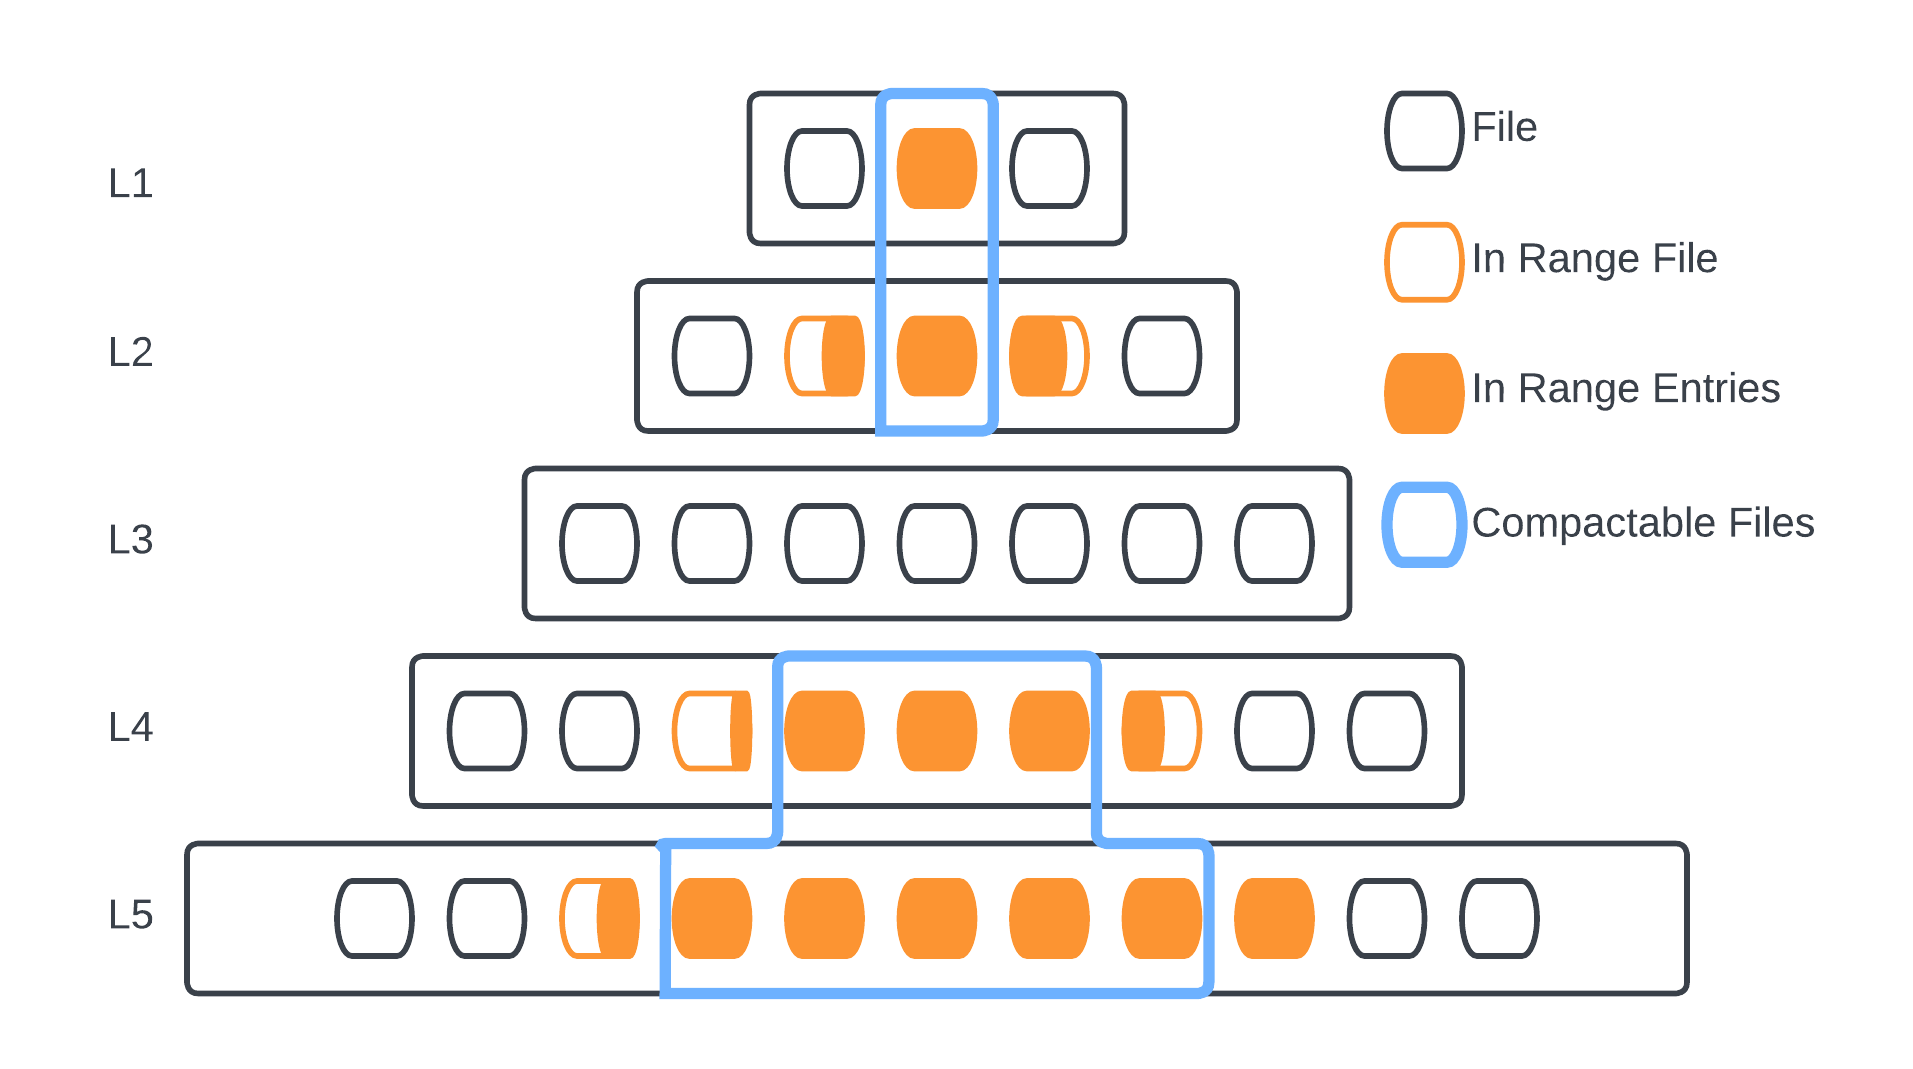
\includegraphics[scale=0.12]{Figures/LSM1.png}
  \caption{Range query driven compaction (a)}
  \label{fig:LSM-tree-a}
\end{figure}

\begin{figure}
  \centering
  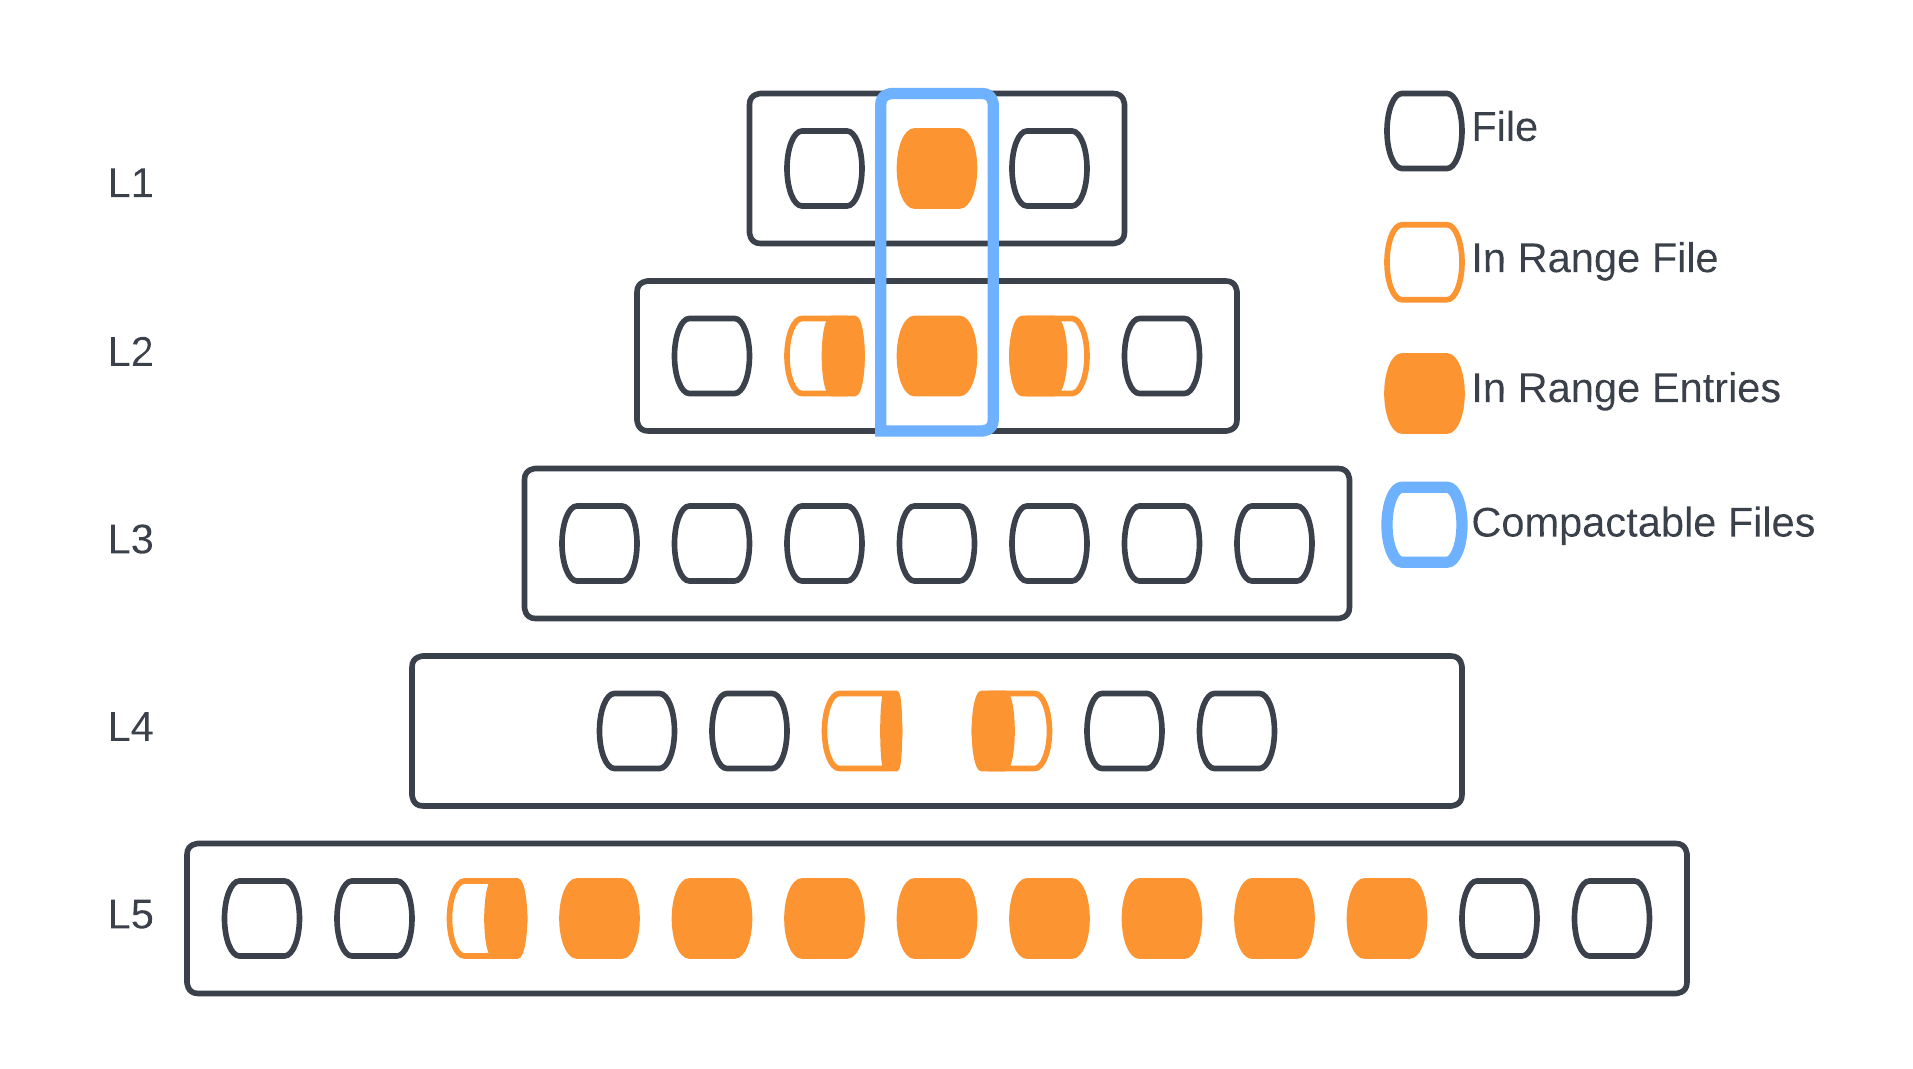
\includegraphics[scale=0.12]{Figures/LSM2.png}
  \caption{Range query driven compaction (b)}
  \label{fig:LSM-tree-b}
\end{figure}

One of the key benefits of this algorithm is that developers who are aware of the potential gains from its implementation can easily integrate it into 
their applications. By understanding the underlying queries and advantages, developers can make informed decisions about when to trigger the algorithm, 
leading to a better overall system performance.

Additionally, the algorithm will eventually support adjustable threshold settings. This feature, once implemented, can allow developers to set a threshold for range query driven compaction, ensuring that 
the process is only initiated when the specified conditions are met. This flexibility enables more precise control over the compaction process, 
ultimately contributing to a more efficient and effective storage system.

This Range Query Driven Compaction algorithm provides a powerful tool for managing data in multi-level storage systems. By offering customizable controls 
and leveraging file metadata for targeted compaction, this algorithm enables developers to optimize their applications' performance and storage efficiency.

\section{Benchmark Explanations}
The experiments were conducted on a machine with the following specifications:

\begin{itemize}
\item Intel Core i7-7700HQ CPU @ 2.8GHz x 4
\item 16GB RAM
\item 512GB HDD
\end{itemize}

The options for RocksDB were set as follows:

\begin{itemize}
  \item Compaction style: Level
  \item Write buffer size: 512KB
  \item Memtable factory: SkipListFactory
  \item Level 0 file num compaction trigger: 2
  \item Target file size base: 512KB
  \item Target file size multiplier: 2
  \item Max background jobs: 4
  \item Max bytes for level base: 512KB
  \item Max bytes for level multiplier: 2
\end{itemize}

\subsection{Results}

Our experiments were conducted using several different workloads. For one particular workload involving 4 million inserts, 6 million updates, 10,000 deletes, 500 range queries, and 40\% selectivity, we present the results in Figures~\ref{fig:Fig-1} and \ref{fig:bargraph}. As shown in Figure \ref{fig:Fig-1}, there is an initial spike due to manual compaction, but the graph then shifts downwards, indicating improved performance. This leads to subsequent range queries becoming more efficient compared to the vanilla approach.

In Figure~\ref{fig:bargraph}, we present statistical measures of the range query performance, including mean, median, maximum, minimum, standard deviation, variance, 95th percentile, and 99th percentile. Our approach shows a higher maximum value compared to the vanilla approach, but the mean, median, 95th percentile, and 99th percentile metrics exhibit significantly better results. These findings suggest that our method delivers a more consistent and improved performance for the majority of range queries, making it a preferable choice for similar workloads.

\subsubsection{Inferences}

Based on the experimental results, the following inferences can be made about the performance of the implemented approach:

\begin{enumerate}
\item The approach performs well when the number of updates is significantly larger than the number of inserts.
\item If there are enough range queries with similar ranges in a workload, the cost of compaction that is performed during the initial range queries can amortized
\end{enumerate}

On the other hand, the approach may not perform as well for workloads with a lower number of updates as compared to inserts, and a high number of range queries with really low selectivity.

\begin{figure}
  \centering
  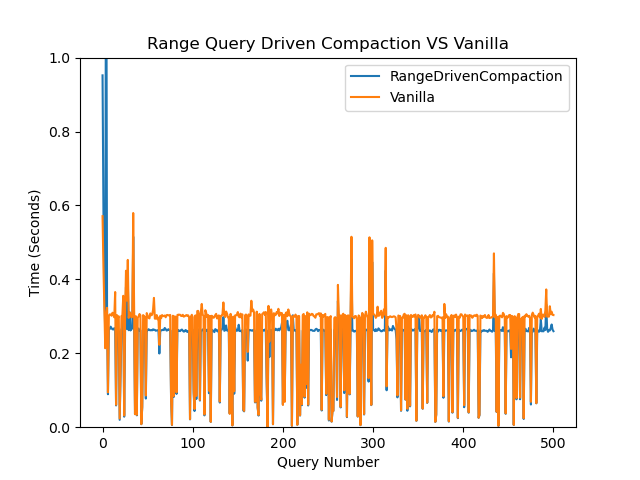
\includegraphics[scale = 0.5]{Figures/c_graph.png}
  \caption{Query driven compaction v/s Vanilla approach (a)}
  \label{fig:Fig-1}
\end{figure}

\begin{figure}
  \centering
  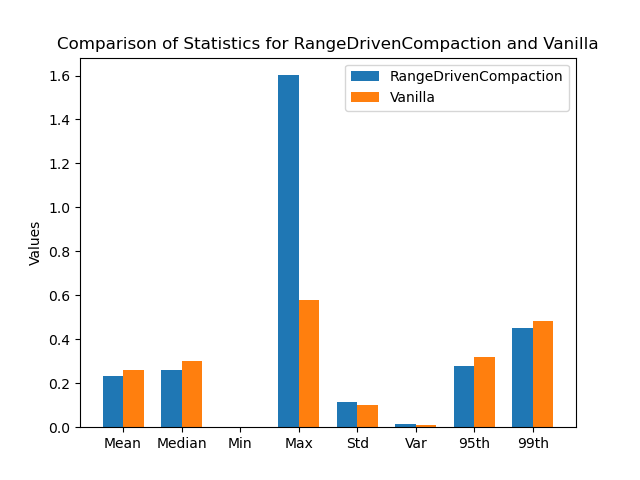
\includegraphics[scale = 0.5]{Figures/bgraph.png}
  \caption{Query driven compaction v/s Vanilla approach (b)}
  \label{fig:bargraph}
\end{figure}

%==============================================================================
\section{Challenges}
In this section, we detail the challenges we faced and our experiences.

\begin{enumerate}
    \item Exploring and Understanding RocksDB: To implement an algorithm to improve the performance of RocksDB for certain workloads, we have delved into the intricacies of RocksDB, an open-source key-value store that already boasts high performance and efficiency for a variety of applications. In order to effectively harness the power of RocksDB, we have studied its core components such as the LSM tree data structure, the compaction process, the process of performing range queries, and the tunable parameters that influence performance. This exploration has proven to be a challenging yet enriching learning experience for us.

    \item Generating Optimal Workloads: One key aspect of our project is the generation of optimal workloads to evaluate the performance of our algorithm. Crafting these workloads has required us to gain an in-depth understanding of RocksDB's performance for different workloads. We have strived to ensure that our workloads are flexible so as to cover all possible scenarios we could. By employing a well-rounded workload generator, we have been able to identify performance bottlenecks and derive valuable insights for tuning and optimizing our algorithm in the future.
\end{enumerate}
% =============================================================================
\section{Future Work}
While our algorithm has demonstrated improved results for update-heavy workloads with frequent range queries, there is still potential for further enhancements.

One area for future work is implementing threshold mechanisms that provide a more granular control over the range-driven compaction algorithm. This could enable more fine-tuned adjustments to the algorithm based on specific workload requirements.

Another area for improvement is optimizing the algorithm to reduce the amount of repeated operations it performs when selecting files for compaction. This could further enhance the efficiency and performance of the algorithm.

In addition, we can explore the possibility of designing an algorithm that uses iterators to perform optimal compactions on the LSM tree, with the aim of improving the performance of range queries. This could provide an alternative approach to the Range Query based Eager Compaction approach we have proposed.

Overall, there are several potential avenues for future research and development in the field of LSM-tree compactions for more efficient range query processing.
% =============================================================================

% =============================================================================
\section{Conclusion}
% =============================================================================
 In this research project, we present a novel approach to perform LSM-tree compactions, focusing on improving the efficiency of range query processing in range operations heavy workloads. We have discussed two potential approaches for this, Eager Compaction based on Range Query and Intelligent Iterator, and presented an algorithm that follows the former approach. We demonstrated the benefits of the algorithm using experimental results. There is still some potential to improve upon these, to further enhance the performance in terms of I/O operations, CPU computation cycles, and storage efficiency, while reducing write and read amplification.
% reference

 \bibliographystyle{unsrt}
 \bibliography{final_project/biblio}


\end{document}